\documentclass[]{article}
\usepackage{amsmath}
\usepackage[]{algorithm2e}
\usepackage{gensymb}
\usepackage{graphicx}
\usepackage{float}

%opening
\title{Report of the computational solution for 1D acoustic wave equation}
\author{Leevi Tuikka, 014583623}

\begin{document}

\maketitle
\pagenumbering{gobble} 

\newpage
\pagenumbering{arabic}

\section{Introduction}
This project implements the computational solution for 1D acoustic wave equation. Acoustic wave equation is the basic equation in seismology, as we consider Earth's crust and upper mantle to deform elastically. In this report, the theory behind the program is handled first, then technical details of the program and results from the program as the last part. \par
In the file structure, video and image files can be found under \texttt{media/} and the source code and the input file under \texttt{src/}.

\section{Theory}

\subsection{Physical and mathematical foundations}

The whole basis of this project lies on one-dimensional scalar wave equation which is second-order partial differential equation. Physically it describes, how wave, i.e. disturbance, advances in a physical medium (string in this case) as a function of time and space. One-dimensional wave equation looks the following
\begin{equation}
	\frac{\partial^2 u\left(x\right)}{\partial t^2}=c^2\frac{\partial^2 u\left(x\right)}{\partial x^2}
\end{equation} 
where $\frac{\partial^2}{\partial t^2}$ is second-order partial time derivative, $\frac{\partial^2}{\partial x^2}$ is second-order spatial derivative, $u(x)$ is the disturbance, $x$ is the only spatial coordinate of the medium and $c$ is the propagation speed of the disturbance, defined by the mechanical properties of the medium. \par
"Disturbance $u\left(x\right)$" might sound a bit abstract as it is, so let us limit wave type to only mechanical waves and particularly longitudinal waves. This wave type advances to same direction as the disturbance is. Therefore, in order to describe disturbance mathematically, no other variables (e.g. angles) than magnitude of the disturbance are needed, so we are really dealing with scalar object. We can also conclude, that as we are dealing with mechanical longitudinal waves producing scalar disturbances, those disturbances manifest as density changes in a continuous medium. Now, by cutting out possible temperature changes and changes of chemical composition of a medium, and looking at changes in mechanical properties leading to density changes, it becomes evident that "disturbance" is actually variation in mechanical pressure. Density variations also leads us to deformation, which poses elastic behaviour in this particular case, if we consider a medium to dense gas or elastic geological material. To relate previous discussion to equation (1), let us define square of the propagation speed
\begin{equation}
	c^2=\frac{K}{\rho}
\end{equation} 
where $K$ is the bulk modulus, which defines how much a medium deforms as a function of stress and $\rho$ is the density. For the sake of clarity, let us define $p\left(x,t\right)\equiv u\left(x,t\right)$, so it matches SI symbol. \par 
Now, as we know what eq. (1) more or less presents, it makes sense to start putting it to some more useful form. Currently, eq. (1) assumes, that disturbance travels somewhere outside of the boundaries of the medium, which needs to be fixed for this project. Therefore we introduce the source term
\begin{equation}
	s=f\left(x,t\right)
\end{equation}
where $f(x,t)$ is some arbitrary function, as a function of place and time. We consider point source, i.e. the source function can "produce non-zero values" only in one spatial point, so source time function can be decomposed into Dirac delta function $\delta\left(x\right)$ and some arbitrary function $g\left(t\right)$ which varies as a function of time
\begin{equation}
	s\left(x,t\right)=\delta\left(x\right)g\left(t\right)
\end{equation}
For this project, we use particular form$^{\left[1\right]}$ of the 1st derivative of Gaussian function for $g\left(x\right)$, so source function becomes the following
\begin{equation}
	s\left(x,t\right)=\delta\left(x\right)g\left(t\right)=\delta\left(x\right)\cdot\left(-8f_0\left(t-t_0\right)e^{-16f_0^2\left(t-t_0\right)^2}\right)
\end{equation}
As we have now defined the source function, complete form of the 1D scalar wave equation with source looks the following
\begin{equation}
	\frac{\partial^2 p\left(x\right)}{\partial t^2}=c^2\frac{\partial^2 p\left(x\right)}{\partial x^2}+s\left(x,t\right)
\end{equation}

\subsection{Discretization}
To be able to transform eq. (6) into program code, it must be transformed from the continuous domain to the discretized domain. For this, let us define some arbitrary discretization point $x_j=j\textrm{d}x$, where $j\in\left[0,j_\textrm{max}\right]$ is the index of the particular discretization point and $\textrm{d}x$ is the grid spacing coefficient, i.e. the distance between two discretization points, which is constant in this project. Also time domain must be discretized, so let us define some arbitrary time step as $t_n=n\textrm{d}t$, where $n\in\left[0,n_\textrm{max}\right]$ is the index of the time step and $\textrm{d}t$ is the length of the time step. Using the previous definitions, pressure at a given place and time can be written
\begin{equation}
	p\left(x_j,t_n\right)=p^n_j
\end{equation}
when eq. (6) becomes with eq. (4)
\begin{equation}
	\frac{\partial^2 p^n_j}{\partial t^2}=c^2_j\frac{\partial^2 p^n_j}{\partial x^2}+\delta_j g^n
\end{equation}
as we demand, that also propagation speed $c$ may vary as a function of space. However, derivatives are still presented in a continuous fashion. By using finite difference method, first-order derivative is defined in the following way
\begin{equation}
	\frac{\partial f\left(x\right)}{\partial x}=\lim\limits_{dx \rightarrow 0}\frac{f\left(x+\textrm{d}x\right)-f\left(x-\textrm{d}x\right)}{\textrm{d}x}
\end{equation} 
In order to deal with the $\lim\limits_{dx \rightarrow 0}$, eq. (9) can be split to backward-difference scheme, central-difference scheme and forward-difference scheme 
\begin{align*}
	\frac{\partial f^-\left(x\right)}{\partial x}&\approx\frac{f\left(x\right)-f\left(x-\textrm{d}x\right)}{\textrm{d}x} \\
	\frac{\partial f^c\left(x\right)}{\partial x}&\approx\frac{f\left(x+\textrm{d}x\right)-f\left(x-\textrm{d}x\right)}{2\textrm{d}x} \\
	\frac{\partial f^+\left(x\right)}{\partial x}&\approx\frac{f\left(x+\textrm{d}x\right)-f\left(x\right)}{\textrm{d}x}
\end{align*}
To pick the best one of these, we can estimate errors by using Taylor series expansion
\begin{equation}
	f\left(x+\textrm{d}x\right)\approx f\left(x\right)+f'\left(x\right)\textrm{d}x+\frac{1}{2}f''\left(x\right)\textrm{d}x^2+O\left(\textrm{d}x^3\right)
\end{equation}
Backward-difference scheme and forward-difference scheme should be symmetrical for some symmetric function, so we can estimate error of both by picking either one and expanding it to Taylor series
\begin{equation*}
	\frac{\partial f^-\left(x\right)}{\partial x}\approx f'\left(x\right)+O\left(\textrm{d}x\right)
\end{equation*}
And Taylor series expansion for the central-difference scheme
\begin{equation*}
	\frac{\partial f^c\left(x\right)}{\partial x}\approx f'\left(x\right)+O\left(\textrm{d}x^2\right)
\end{equation*}
so it is evident that central-difference scheme converges fastest, i.e. gives best solution as the $\textrm{d}x\rightarrow 0$. \par
Now, to construct discretized form for the 2nd order derivative, we would like to use of course central-difference scheme. This can be done by using backward-difference and forward-difference schemes of once differentiated function, since we are trying to find the slope of the slope. Now, the central-difference scheme for the second order derivative would be 
\begin{equation*}
	\frac{\partial^2 f^c\left(x\right)}{\partial x^2}\approx \frac{\frac{\partial f^+\left(x\right)}{\partial x}-\frac{\partial f^-\left(x\right)}{\partial x}}{\textrm{d}x}=\frac{f\left(x+\textrm{d}x\right)-2f\left(x\right)+f\left(x-\textrm{d}x\right)}{\textrm{d}x^2}
\end{equation*}
And plugging this to eq. (6) we get
\begin{equation}
	\frac{p_j^{n+1}-2p_j^n+p_j^{n-1}}{\textrm{d}t^2}=c^2_j\left(\frac{p_{j+1}^n-2p_j^n+p_{j-1}^n}{\textrm{d}x^2}\right)+\delta_j g^n
\end{equation}
In order to find $p_j^{n+1}$, i.e. value for the pressure on the next time step at some spatial point, eq. (11) must be rearranged to form
\begin{equation}
	p_j^{n+1}=c_j^2\frac{\textrm{d}t^2}{\textrm{d}x^2}\left(p^n_{j+1}-2p^n_j+p^n_{j-1}\right)+2p^n_j-p_j^{n-1}+\textrm{d}t^2\delta_j g^n	
\end{equation}

\subsection{Source}
Mathematically the source function eq. (5) is integrated over time. Therefore the waveform should Gaussian function
\begin{equation}
	-8 f_0\int\left(t-t_0\right)e^{-16f_0^2\left(t-t_0\right)^2}=\frac{e^{-16f_0^2\left(t-t_0\right)^2}}{4f_0}
\end{equation}
which looks graphically the following
\begin{center}
	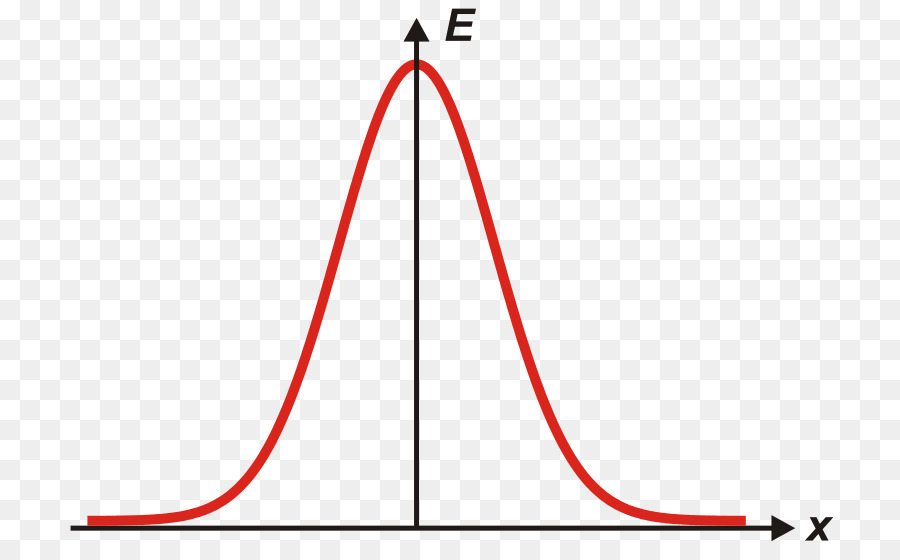
\includegraphics[width=1.0\linewidth]{gaussian}
\end{center}


\newpage

\section{Program code and technical details}

\subsection{Python}
The program code was developed by using 3.6 version of Python, however it should have backward and forward compatibility to all Python 3.x versions. Implementation employs \texttt{numpy}, \texttt{matplotlib}, \texttt{math} libraries which should be included in Python standard libraries.

\subsection{Instructions}
Main functionality of the code is located in \texttt{main.py} file and class definitions to \texttt{class\_defs.py} file. In order to run the program, run the following line on command line \\
\texttt{\$ python3.6 main.py} \\
and the program first prints the input values to the terminal and after execution it opens a new window in order to plot results on $x-t$ domain. Quality of the image may vary but the program also saves the plot to file \texttt{x\_t\_plot.png} which should show the plot as intended.

\subsection{Pseudocode}
begin(); \\
\\
import libraries; \\
\\
input\_file = open("\textbf{input\_file.txt}"); \\
\\
\textit{\# read input parameters to Input class structure}; \\
input\_values = read\_file(input\_file); \\
\\
\textit{\# create Source class object} \\
source = create\_source(source\_id, frequency); \\
\\
\textit{\# init discretization point, propagation speed, density and bulk modulus arrays} \\
points = []; \\
c = []; \\
density = []; \\
K = []; \\
\\
\textit{\# set right values of c, density and K for each point} \\
c = input\_values.get\_c(); \\
density = input\_values.get\_density(); \\
K = input\_values.get\_K(); \\
\\
\textit{\# add Point class objects to points array and set values for them} \\
\textbf{for} i = 0, i $<$ input\_values.get\_n\_points(), i++; \\
\indent points.append(add\_point(i, K[i], density[i], c[i], p=0.0, input\_values)); \\
\indent \textit{\# allocate array for each point to store p values over time steps} \\
\indent points[i].allocate\_t\_array(input\_values.get\_timesteps()); \\
\\
\textit{\# start looping over time steps}; \\
\textbf{for} t = 0, t $<$ input\_values.get\_timesteps(), t++; \\
\indent \textit{\# loop over points at every time step, expect at boundaries} \\
\indent \textit{\# since points on boundaries don't have j+1 or j-1 points} \\
\indent \textbf{for} j = 1, j $<$ input\_values.get\_n\_steps() - 1, j++; \\
\indent \indent \textit{\# calculate value for source if in the source point} \\
\indent \indent \textbf{if} j == source.get\_id(); \\
\indent \indent \indent s = source.calculate(t, dt); \\
\indent \indent \textbf{else}; \\
\indent \indent \indent s = 0; \\
\indent \indent \textit{\# calculate $p^{n+1}$ for each point} \\
\indent \indent points[i].set\_p\_t(c[n]**2 * (input\_values\_get\_dt()**2 / input\_values\_get\_dt()**2) \\
\indent \indent *(points[i+1].get\_p\_t(t) - 2*points[i].get\_p\_t(t) + points[i-1].get\_p\_t(t)) \\
\indent \indent + 2*points[i].get\_p\_t(t) - points[i].get\_p\_t(t-1) + input\_values.get\_dt()**2*s); \\
\\
\textit{\# plot p(t) values from point array over x-t domain} \\
plot(points[i]); \\
\\
end();

\subsection{Classes}
Implementation was done using Python classes for several functionalities. These include
\begin{itemize}
	\item \textbf{Input}: This class structure handles input parameters. First, Input object is initialized by using input parameter variables. Therefore setter functions are not needed, since all the variables are set in the initialization stage. Propagation speed \texttt{c} is calculated in the initialization based on the bulk modulus \texttt{K} and the density \texttt{density}. Only other functionalities in the Input class are getter functions, which are used at any point where input parameters need to be used. 
	
	\item \textbf{Point}: This class deals with single discretization points. Each point has properties: the spatial index \texttt{id}, the bulk modulus \texttt{K}, the density \texttt{density}, the propagation speed \texttt{c} and pressure array \texttt{p\_t[]} over time steps. Point class structure contains setter and getter functions for each variable. It also contains \texttt{solve\_p\_t()} function which solves $p^{n+1}_j$ based on the eq. (12). For debugging purposes, \texttt{print\_point()} function exists, it prints properties of a certain Point object when called. In the beginning of the program, all the Point objects are initialized and appended to a array. Later on in the time step loop, each point is accessed at every time step and $p^{n+1}_j$ is computed by using class functionalities.
	
	\item \textbf{Source}: This class controls the source behaviour. The only variable that Source class object has, is spatial index \texttt{source\_id} defining the source location. Source object is initialized in the beginning of the program by using \texttt{source\_id}. Then it is accessed at every time step by Point objects, which check if current discretization point is the location of the source. If so, then value of the source function is computed as a function of time and the frequency by using \texttt{s\_t()} function and then passed to \texttt{solve\_p\_t()} function.
\end{itemize}

\section{Results}

\subsection{Parameters and different scenarios}
Program implementation allows to use 1-3 different regions in the simulation, i.e. three different materials. Placement and width of the regions are controlled by the \texttt{regions} parameter which defines number of the regions, whereas the \texttt{interface1\_id} defines interface between material 1 and material 2, and the \texttt{interface2\_id} defines interface between material 2 and material 3, assuming that three regions are used. Accordingly, if two are used, only \texttt{interface1\_id} is needed and in the case of one regions, no interface is needed. \par
All the input parameters are defined in the input file. By default, the material 1 has properties of air at 1 atm, the material 2 has bulk modulus of the material 1 and the density two times of material 1, the material 3 has bulk modulus of the material 1 and the density twenty times of material 1. Parameter \texttt{t\_steps} defines the number time steps and \texttt{n\_steps} defines number of discretization points. Product of these two parameters should be somewhere between $9\cdot 10^6-25\cdot 10^6$ for convenient run times and file sizes for output files. \par
Picking suitable values for the time step \texttt{dt} and the grid spacing \texttt{dx} was rather important and challenging part. If \texttt{dt} is too large, program can't catch all the smallest time-wise developments, e.g. regarding the source. Let us have the frequency of the source \texttt{freq} and time step \texttt{dt}, so period of source oscillation is \texttt{T$=1/$freq} and program is able to catch \texttt{T$/$dt} "data points" from the source. For the source frequency, I picked 20 Hz (which roughly gives the biggest amplitude for eq. (5)) and I thought that 200-300 data points from the source should be enough, so \texttt{dt}$=0.2\cdot10^{-3}$ seconds is suitable time step, since it gives 250 data points from the source. Selected \texttt{dt} also works fine in the respect of other things, as long as \texttt{dx} is suitable. Parameter \texttt{dx} can't be too large or otherwise the computational $x$ domain can't transmit wave having relatively short wavelength. Now, considering material 1, wavelength in it is $\lambda=343\;\textrm{ms}^{-1}/20\;\textrm{Hz}=17.15$ meters, so to distribute one period over roughly 100 discretization points, I picked \texttt{dx}=0.1 meters. Also the ratio (\texttt{dt}/\texttt{dx})$^2$ must be big enough. For some reason, ratios less than $10^{-7}$ seems to lead weird disturbances in the waveform. Potentially this happens because last three terms in the eq. (12) become too dominant. The source function in the eq. (5) contains also time offset parameter \texttt{t0}, which defines when the source starts vibrating. Just by experimenting I picked \texttt{t0}=0.04 seconds, smaller values caused disturbances. 

\subsection{Reflections and refractions}
When a wave hits an interface separating two different materials, some portion of it reflects back to its incident direction and rest of it refracts to a new material. These portions are defined by the incident angle and mechanical properties of the two media. However, as we are dealing with one-dimensional case, the incident angle is always $90\degree$. Therefore, only mechanical properties, or to be exact, only propagation velocities matter. Reflection coefficient$^[2]$ defines how large portion of the amplitude (or actually energy) will be reflected to incident direction
\begin{equation}
	R=\frac{c_2-c_1}{c_2+c_1}
\end{equation}
where $c_2$ is the propagation velocity in the second medium and $c_1$ is the propagation velocity in the first medium. On the boundaries, we have set $p^{n+1}_j=0$, so $c_2=0$ on the boundary points and outside of the computational domain which leads to $R=-c_1/c_1=-1$. Physically this means, that the whole wave is reflected back but the amplitude is flipped, i.e. if wave having amplitude $A$ hits the boundary, it will be reflected back having amplitude $-A$ and vice versa. 

\subsection{Quantifying the propagation velocity}
In order to confirm that the program actually works, we can compare propagation velocity that has been given as a parameter, and propagation velocity which is quantified graphically from the output plot. Since the velocity is generally
\begin{equation}
	v=\frac{\textrm{d}x}{\textrm{d}t}
\end{equation}
but we can't use continuous derivatives here, let us define the propagation speed in the following way
\begin{equation}
	c=\frac{x(t_2)-x(t_1)}{t_2-t_1}
\end{equation} 
where $x(t_2)$ is the location of the crest at time $t_2$ and $x(t_1)$ is the location of crest at time $t_1$.

\subsection{Example cases}
\subsubsection{A homogeneous medium}
The first case was run only by using one regions, i.e. one material. For the number of discretization points I used 2000 points and 4000 time steps. Source was located in the middle, $x_j=1000$. As an output the following $x-t$ plot was obtained. \newpage

\begin{figure}[h!]
	\centering
	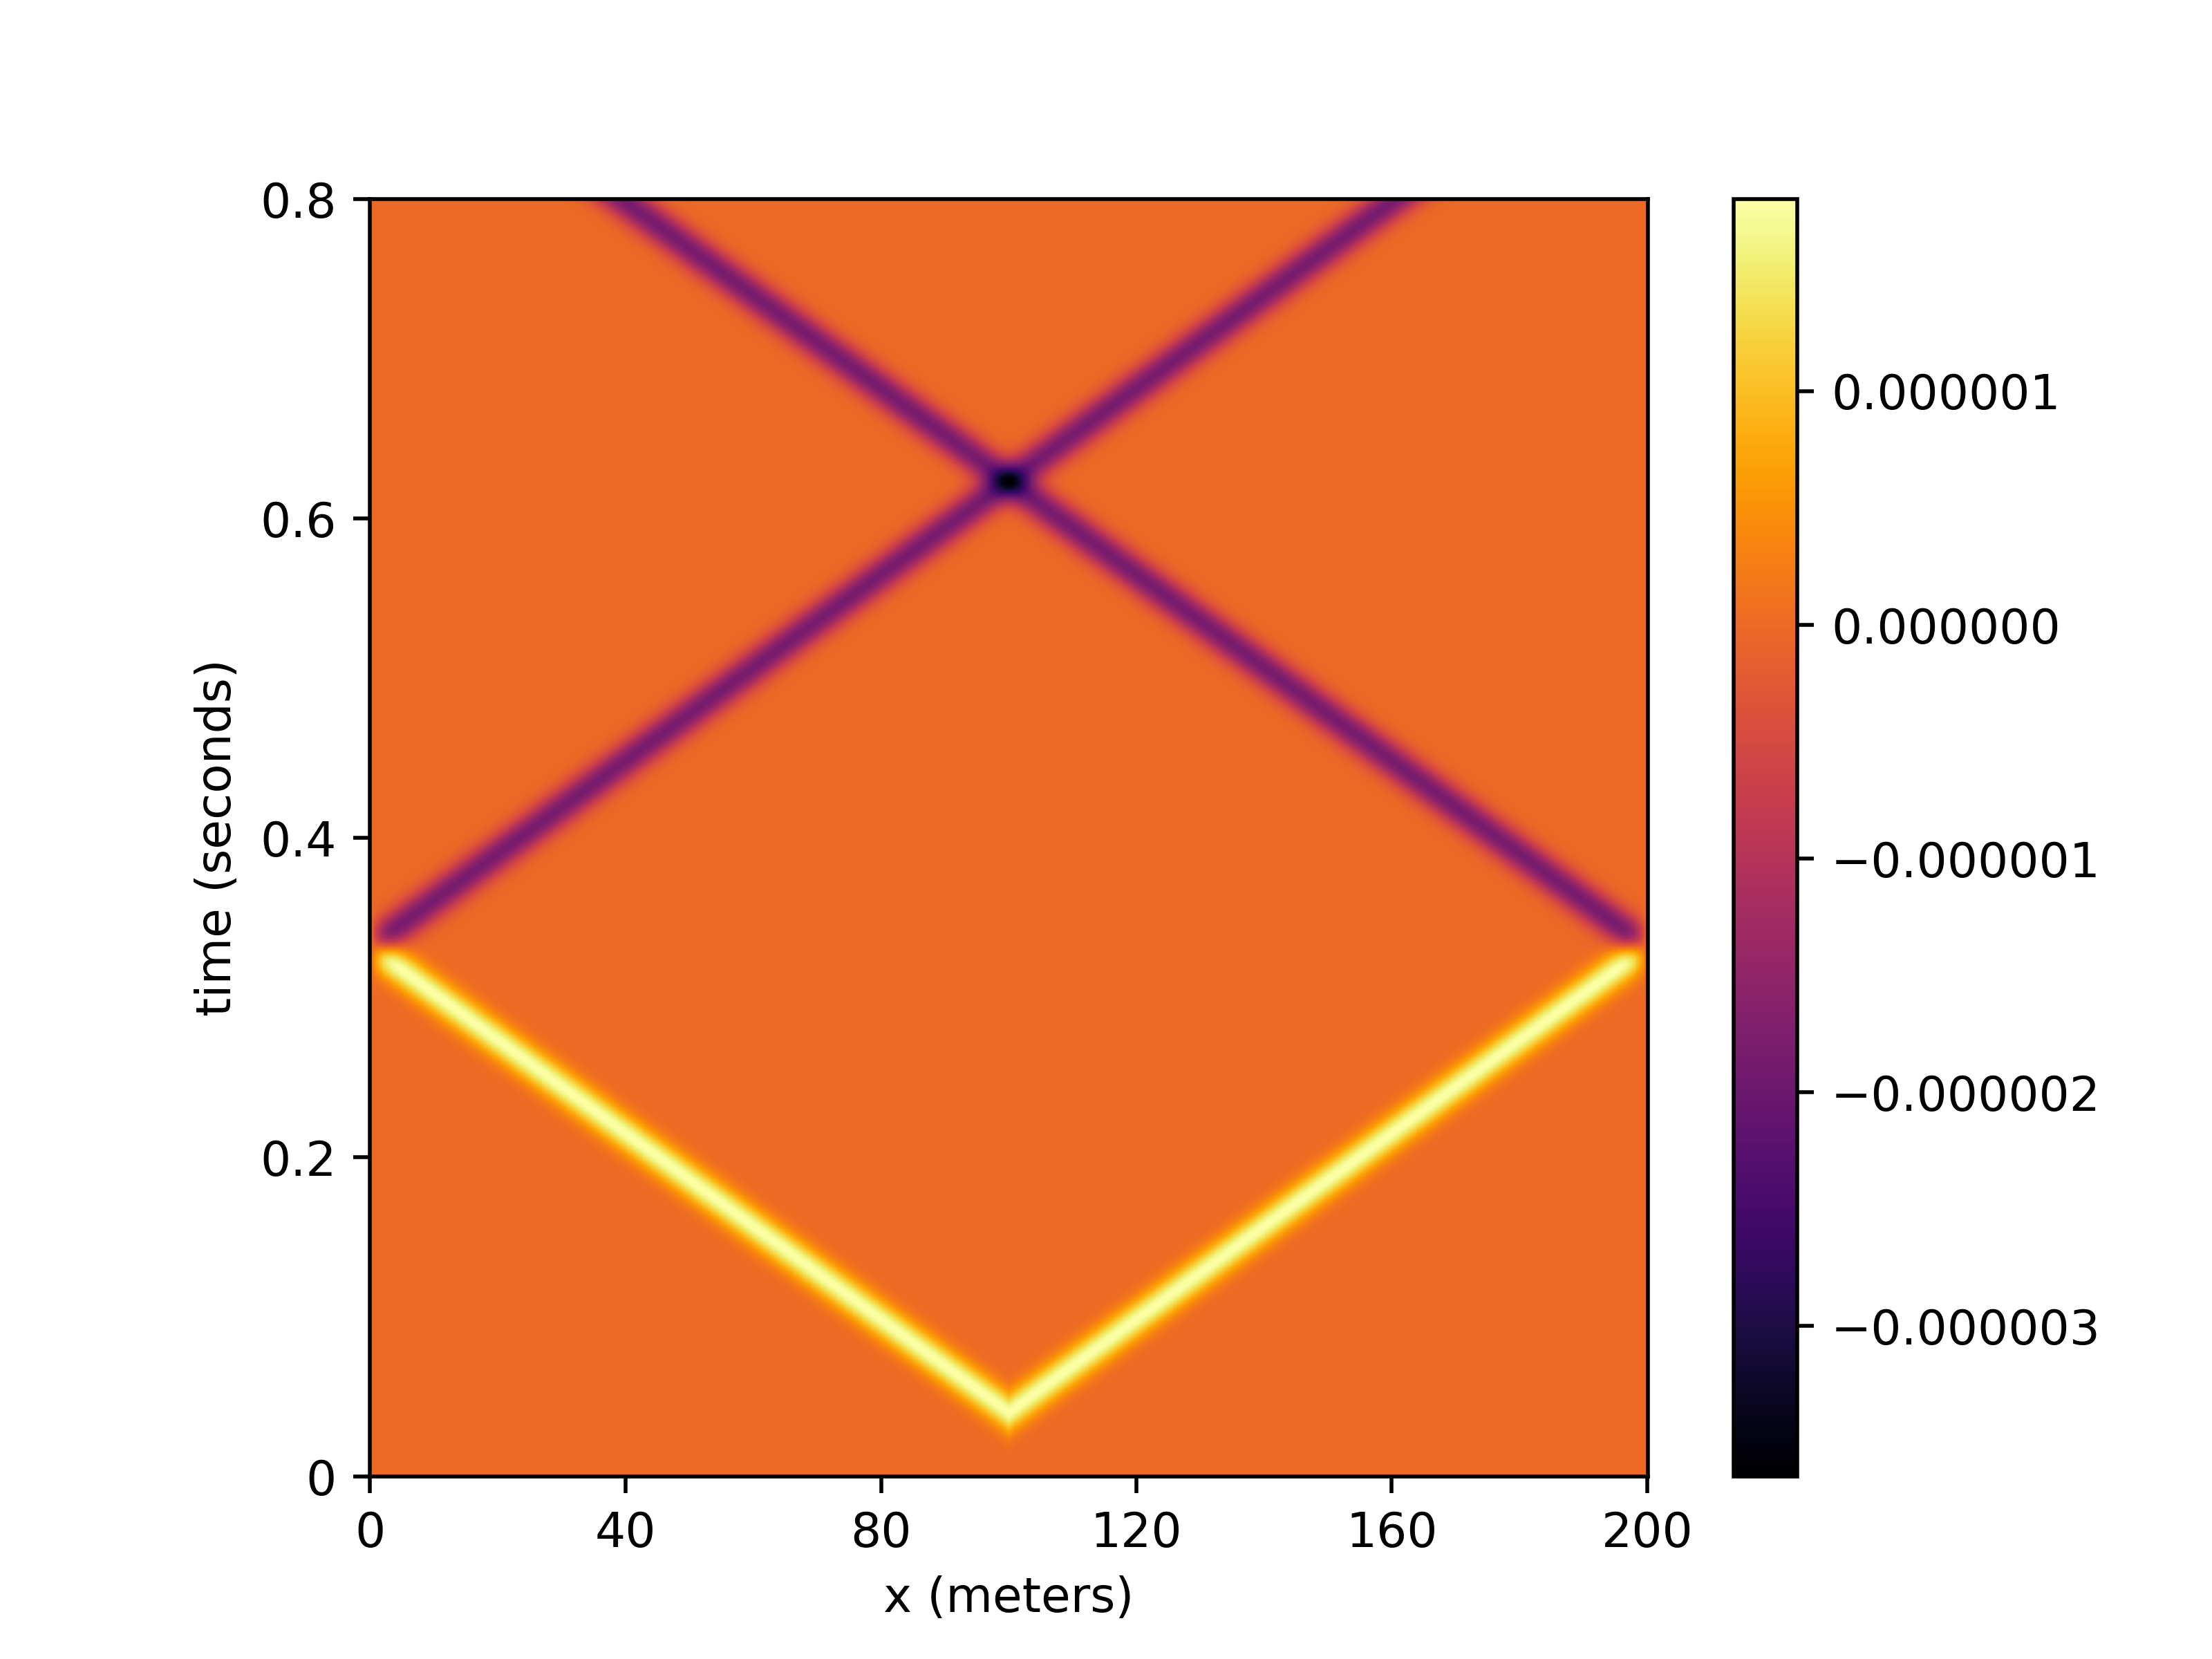
\includegraphics[width=1.0\linewidth]{media/plot_1_region}
	\caption{Colourbar presents the range of the pressure variation in pascals. Black dot at 0.6 seconds is the superposition of the two waves, i.e. the amplitude is $-2A$.}
	\label{fig:plot1region}
\end{figure}

From this plot we are able estimate propagation speed. Let us pick roughly $t_1=0.04$ s, so $x(t_1)=100$ m. Wave reaches boundaries roughly at $t_2=0.34$ s and $x(t_2)=0$ m. This gives propagation speed $c=100\;\textrm{m}/(0.34-0.04)\;\textrm{m}=333.333...\;\textrm{m/s}$ which is quite close to the exact value 343 m/s, so I would conclude that the program works as it should. Also, at the boundaries, wave is flipped upside down, which is expected as well. Behaviour of the wave can be seen on video file \texttt{animation\_1\_region.mp4} and the high-resolution plot is in file \texttt{plot\_1\_region.png}.
 

\subsubsection{Two regions}
The second case was run by using two regions, i.e. two materials. For the number of discretization points I used 4000 points and 4000 time steps. Source was located at $x_j=1000$ and the interface at $x_j=2000$. In this case, the wave is reflected at the interface. The following is snapshot of the video file \texttt{animation\_2\_regions.mp4}, right away after the reflection (higher resolution image can be found \texttt{media/reflection.png})
\begin{center}
	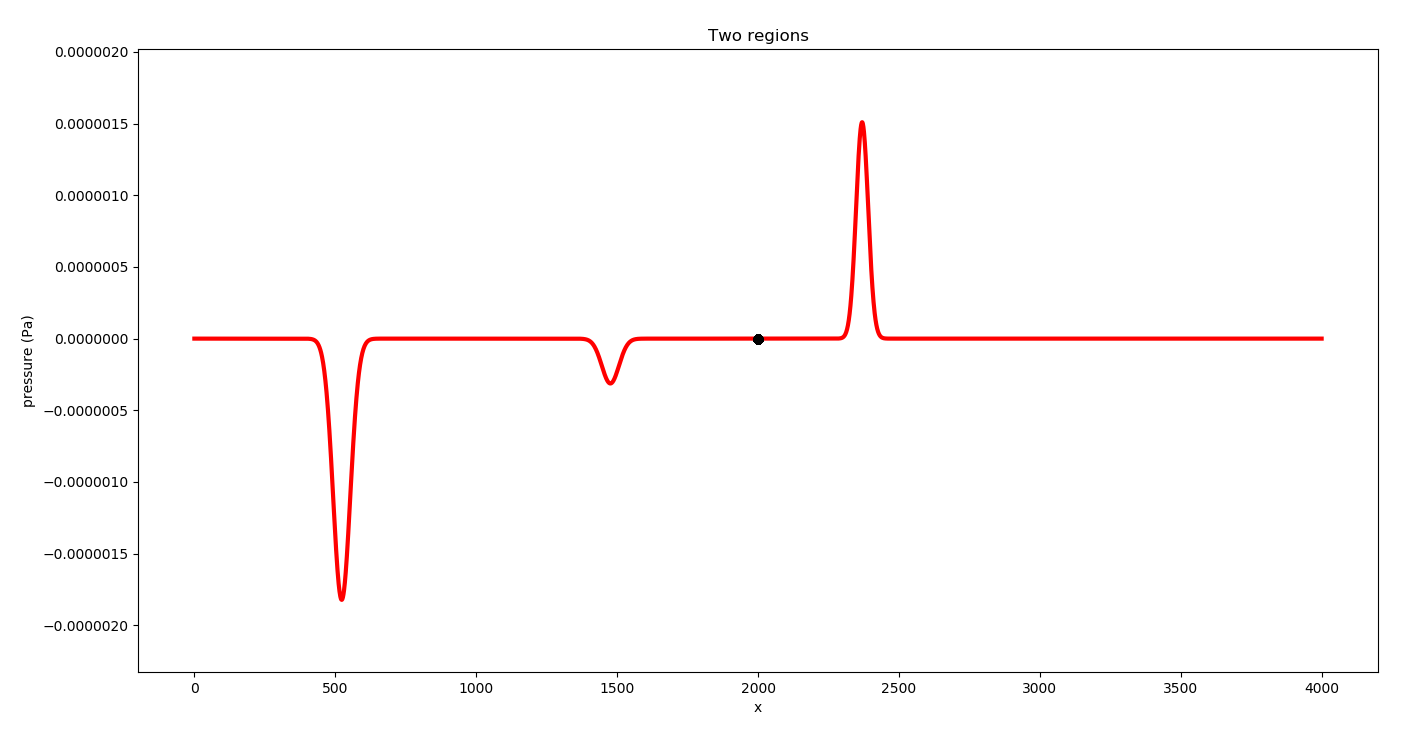
\includegraphics[width=1.0\linewidth]{media/reflected}
\end{center}
As the medium on the left of the interface has propagation speed $c_1=343$ m/s and the medium on the right of the interface has propagation speed $c_2=\sqrt{141200\;\textrm{Pa}/2.4004\;\textrm{kg/m}^3}=242.536...$ m/s. Now, by employing eq. (13), let us compute the reflection coefficient
\begin{equation}
	R=\frac{242.536\;\textrm{m/s}-343\;\textrm{m/s}}{242.536\;\textrm{m/s}+343\;\textrm{m/s}}=-0.172...
\end{equation}
i.e. 17.2\% of the amplitude should be reflected back. By estimating amount of reflection graphically, the undisturbed amplitude is $1.8\cdot 10^{-6}$ Pa, whereas the reflected the reflected amplitude is roughly $0.3\cdot 10^{-6}$ Pa, so graphically estimating $0.3/1.8=16.666...\%$ of the amplitude was reflected, which is again quite a good result. Also the $x-t$ domain plot (high-resolution version \texttt{media/plot\_2\_regions.png}) looks the following \\
\begin{figure}[H]
	\centering
	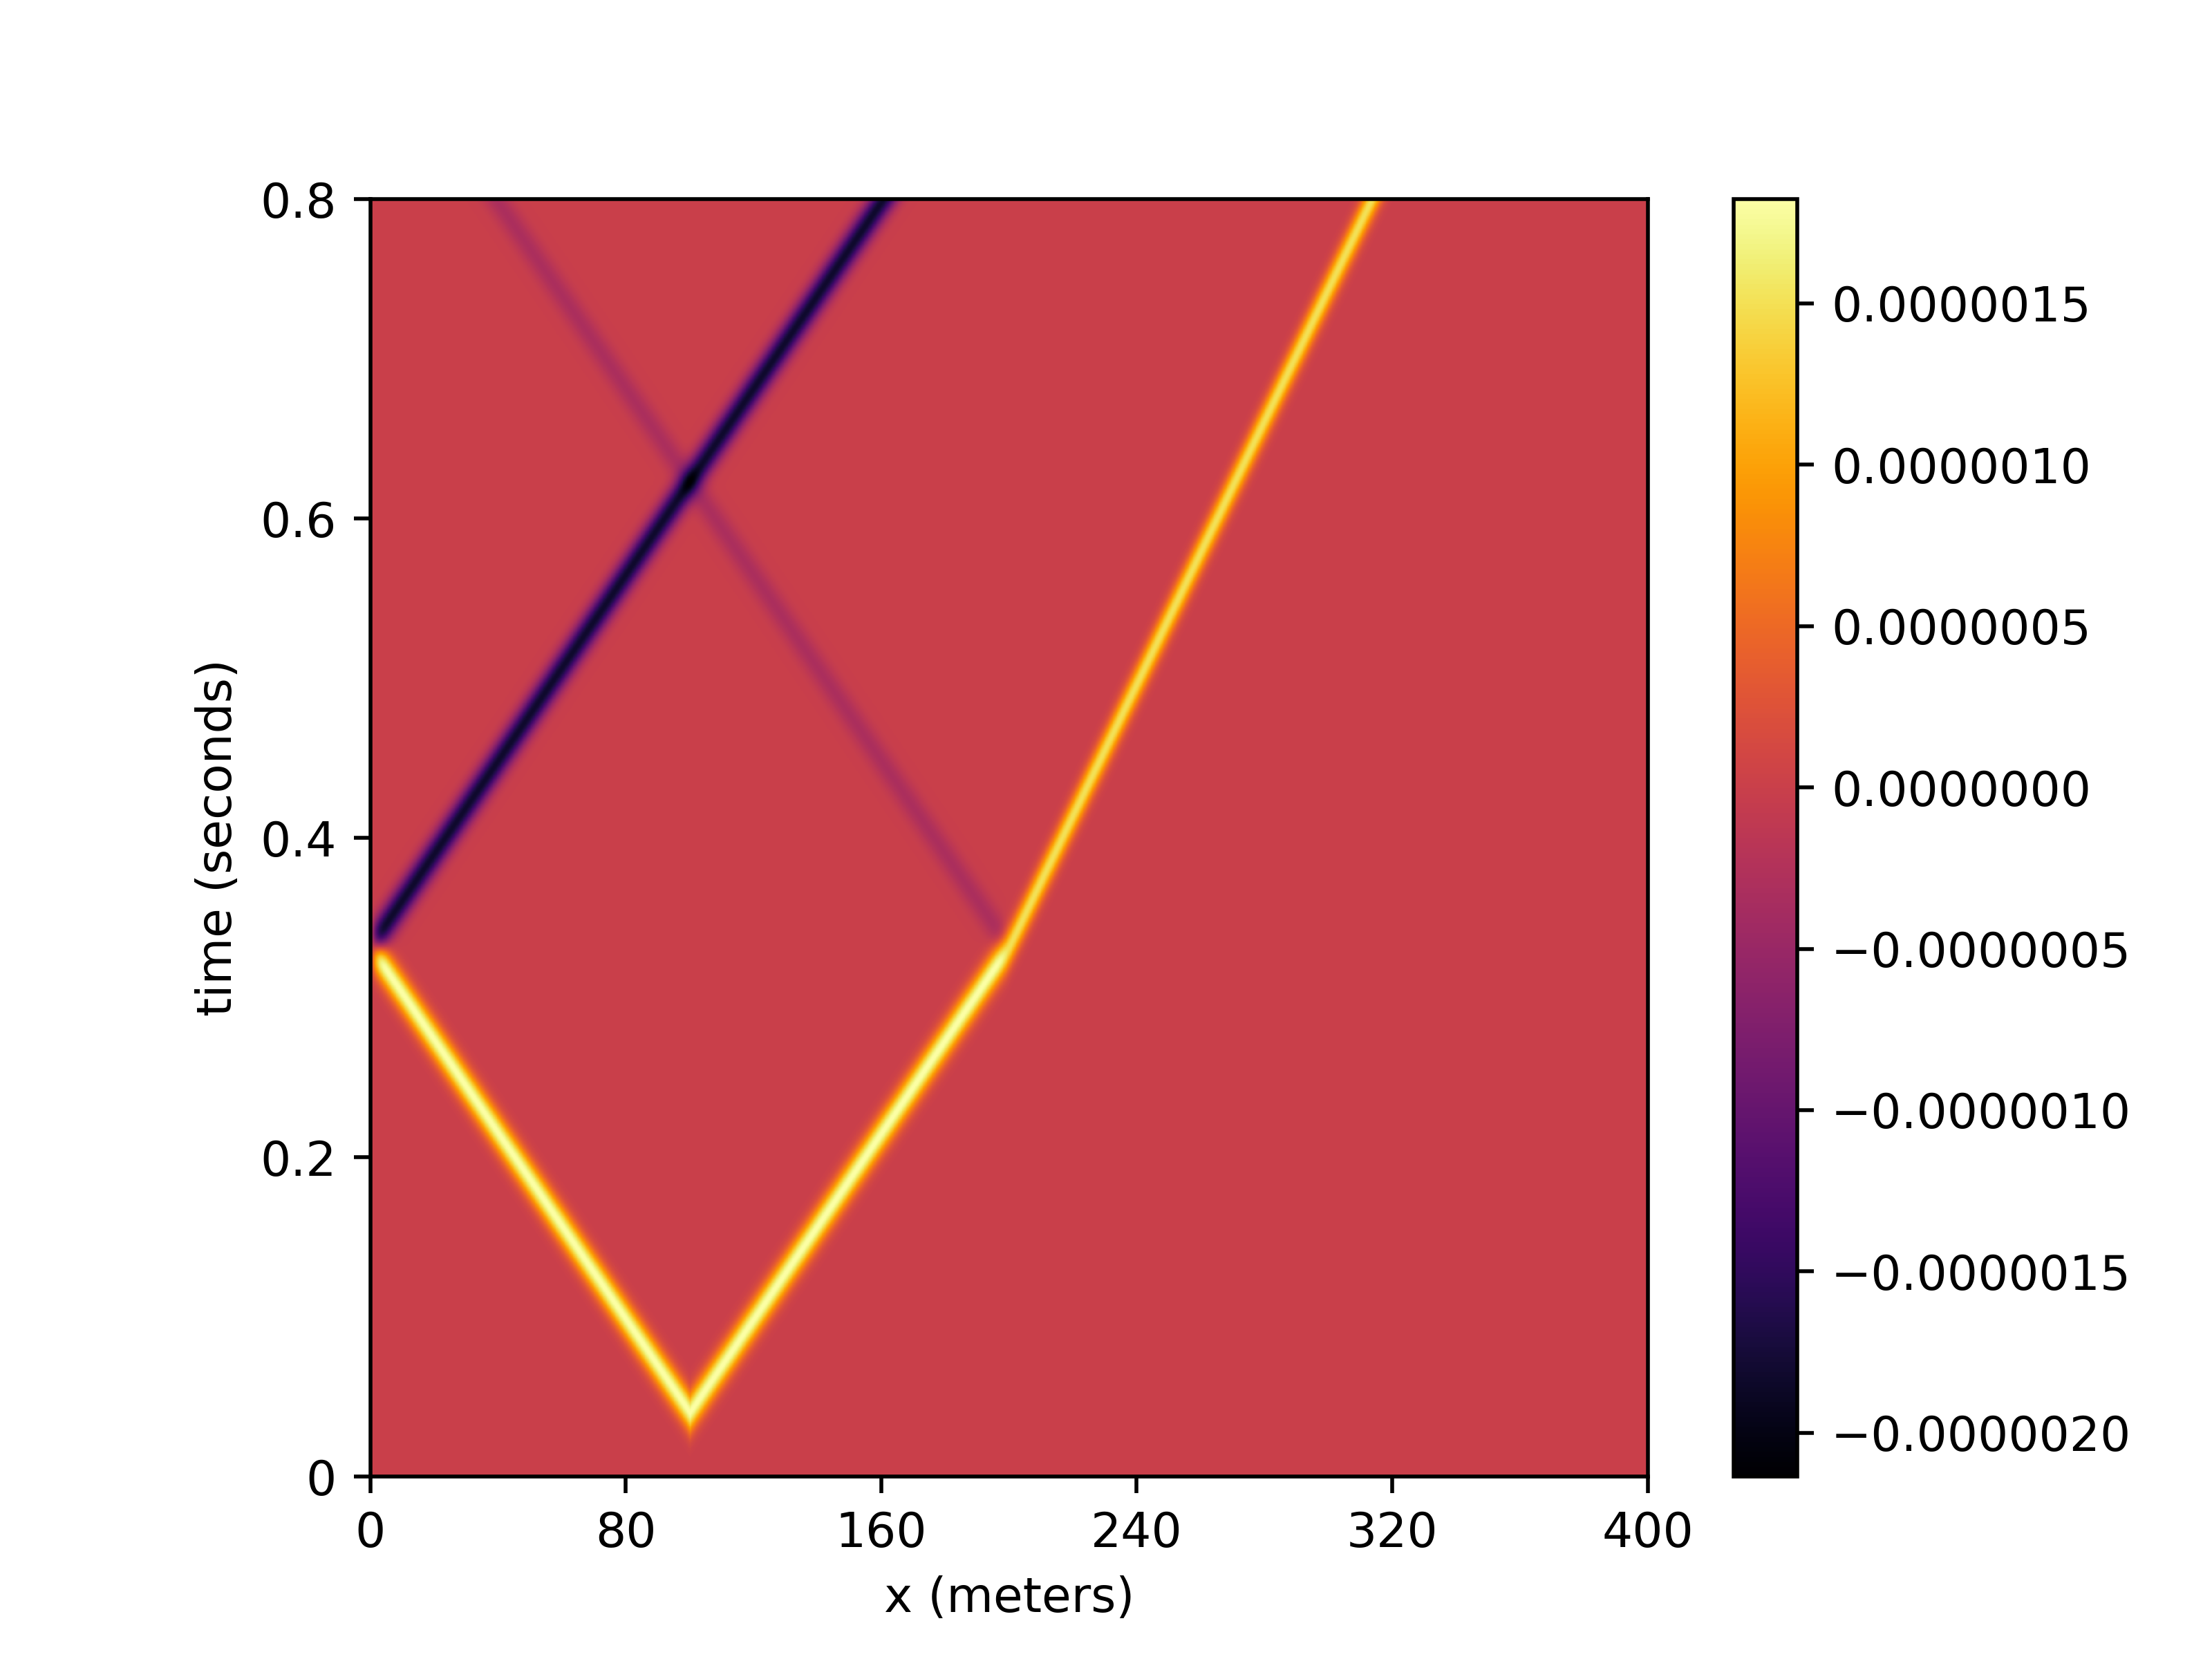
\includegraphics[width=1.0\linewidth]{media/plot_2_regions}
	\caption{Colourbar presents the range of the pressure variation in pascals.}
	\label{fig:plot2regions}
\end{figure} 
 
\subsubsection{Three regions}
The third case was run by using three regions, i.e. three materials. For the number of discretization points I used 4000 points and 4000 time steps. Source was located at $x_j=1500$, the interface 1 at $x_j=2000$ and the interface 2 at $x_j=3000$. This simulation doesn't pose any useful example but rather demonstrates chaotic nature of the wave travelling in multiple media, which can been seen also on video \texttt{animation\_3\_regions.mp4}. The $x-t$ domain plot (high-resolution version \texttt{media/plot\_3\_regions.png}) looks the following 
\begin{figure}[H]
	\centering
	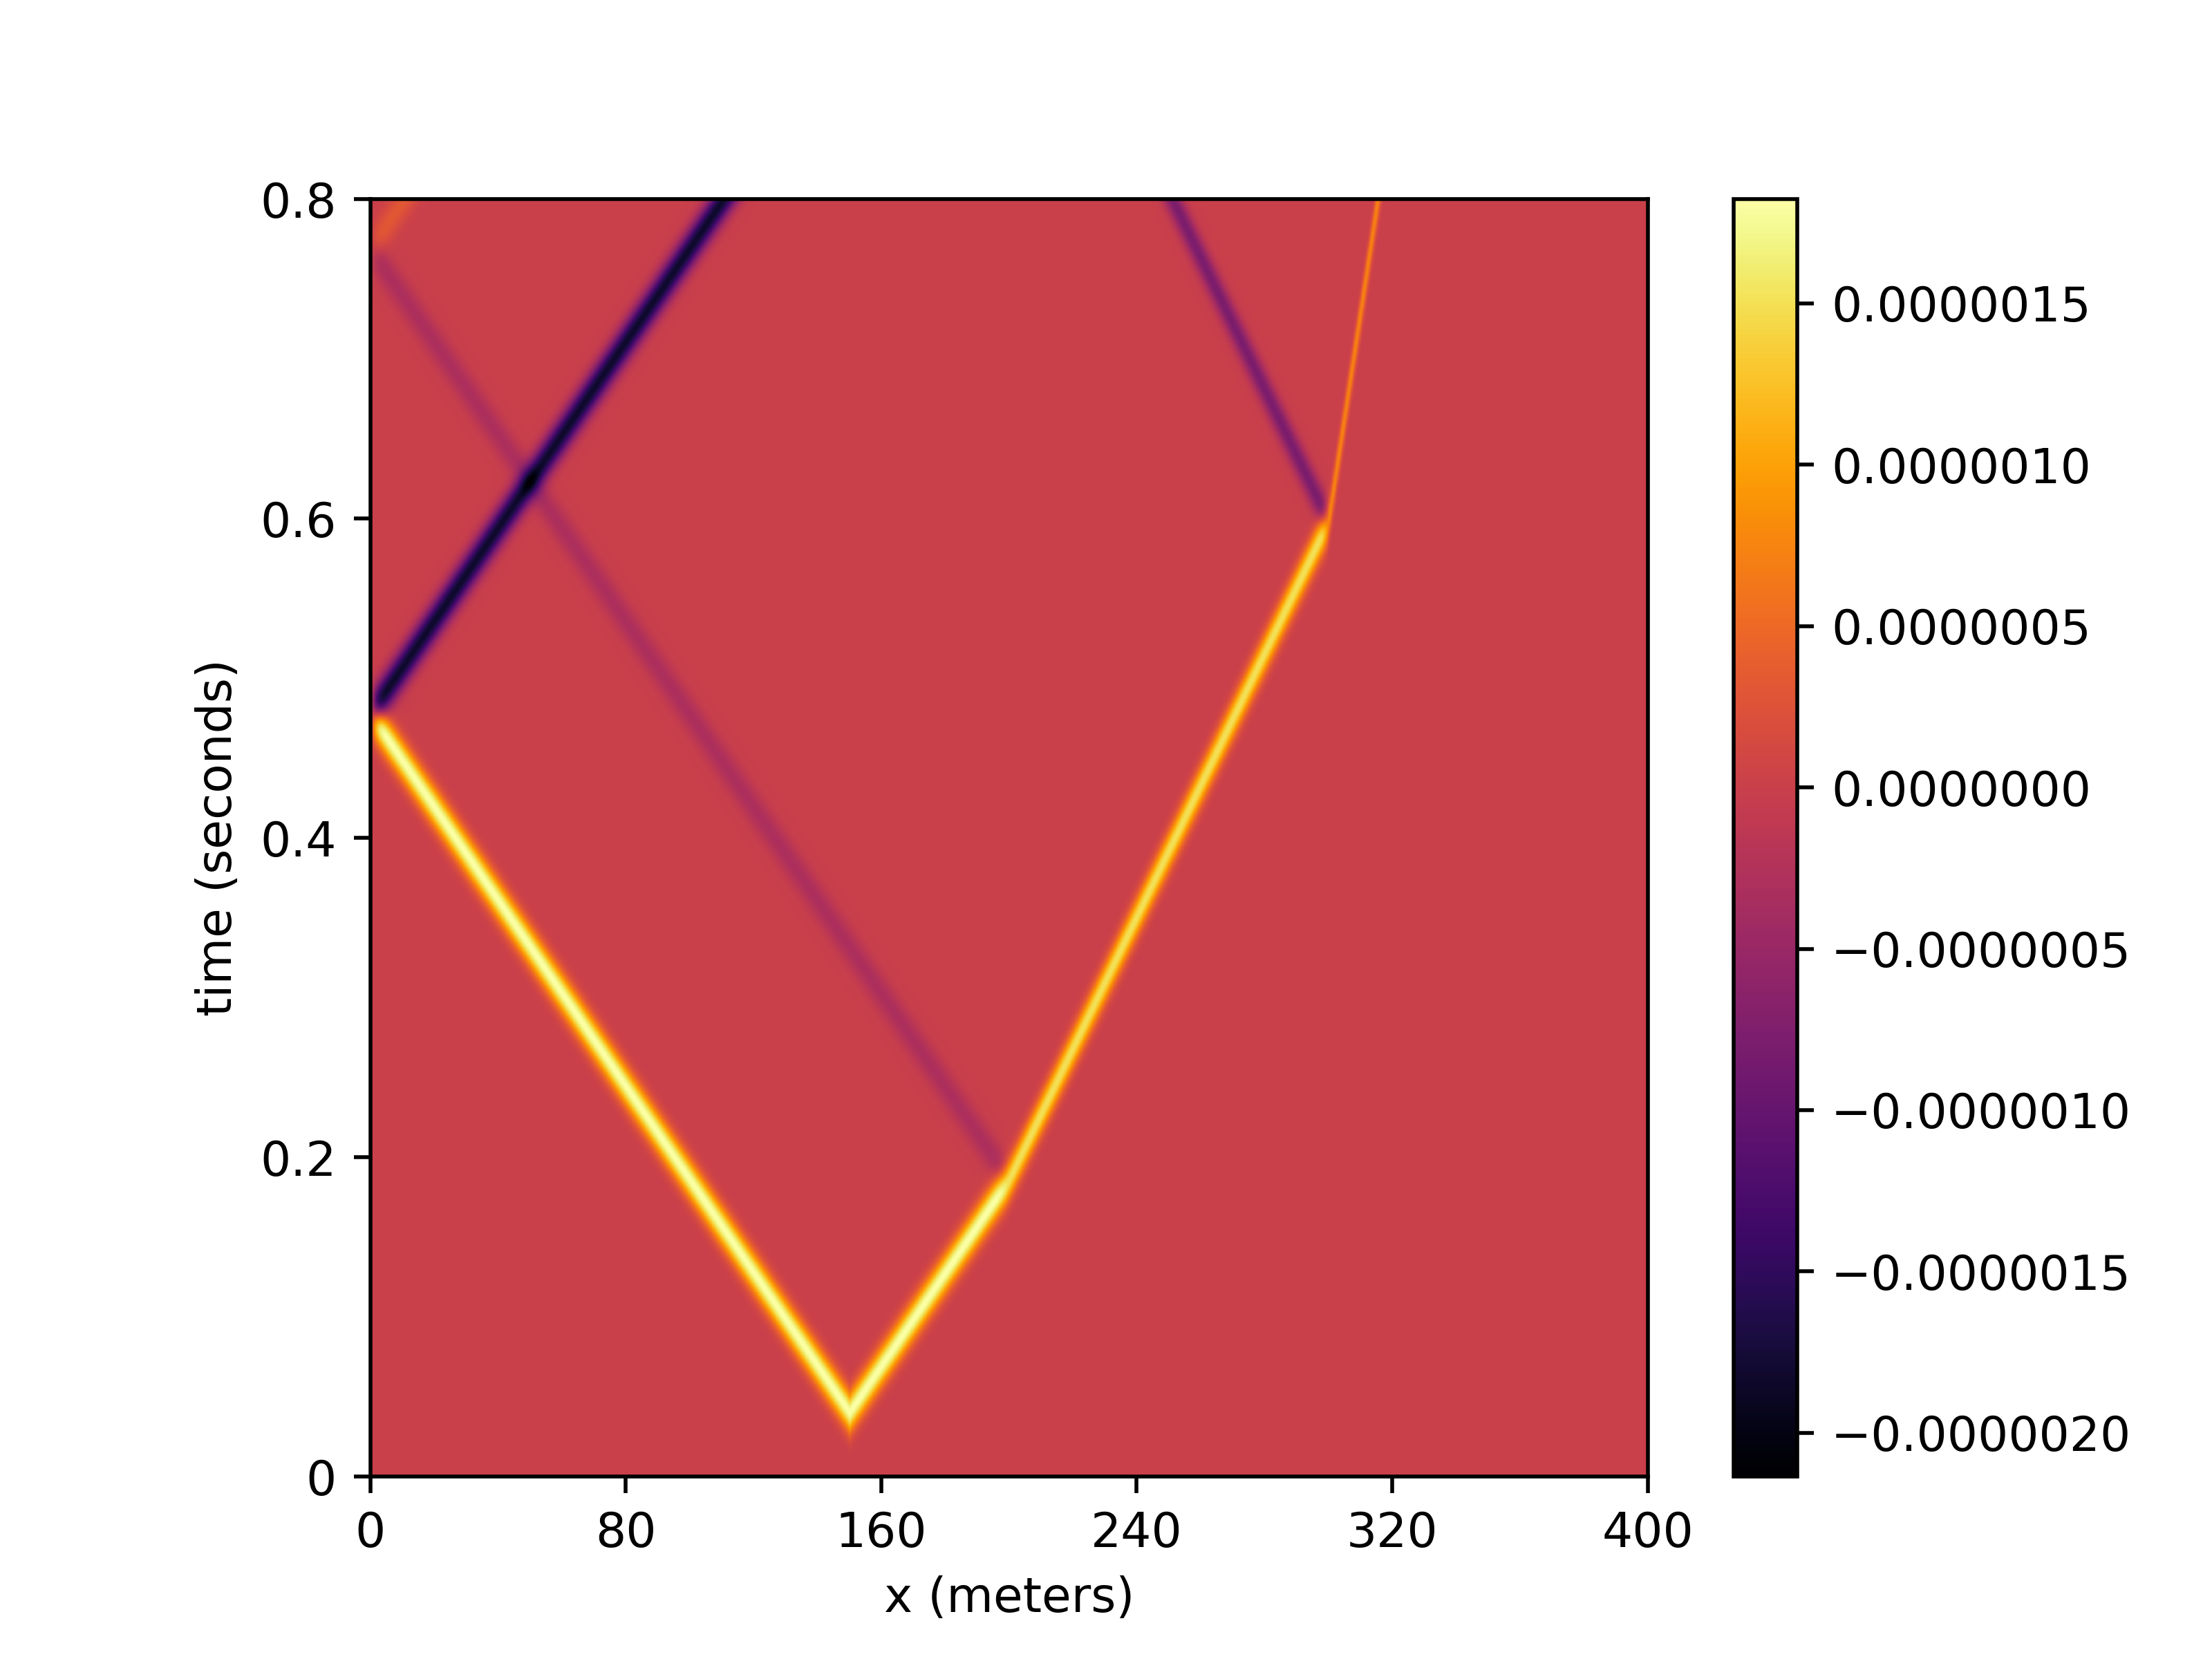
\includegraphics[width=1.0\linewidth]{media/plot_3_regions}
	\caption{Colourbar presents the range of the pressure variation in pascals.}
	\label{fig:plot3regions}
\end{figure}
This however demonstrates quite well, how the wavelength is defined by the density, as the wavelength decreases drastically when wave passes from density 2.4004 kg/m$s^2$ to 24.004 kg/m$s^2$ at $x_j=3000$.

\section{References}
[1]  Igel, H. (2016) Computational Seismology: A Practical Introduction. 1st edn. Oxford: Oxford University Press. doi: 10.1093/acprof:oso/9780198717409.001.0001. \\

\noindent [2] Shearer, P. M. (2009) Introduction to Seismology. 2nd edn. Cambridge: Cambridge University Press. doi: 10.1017/CBO9780511841552.


\end{document}
